\documentclass{article}
\author{Maria Alejandra Arias Jaimes}
\usepackage[utf8]{inputenc}
\date{20 de julio de 2017}
\title{Métodos Computacionales. Tarea 3}
\usepackage[utf8]{inputenc}
\usepackage{amsmath, amssymb, graphicx}
\usepackage[utf8]{inputenc}

\frenchspacing

\newcommand{\JournalIssue}[1]{%
                \hfill \textsc{20 de Julio de 2017}
                \par \normalsize \normalfont}

\newcommand{\JournalName}[1]{%
                \begin{center}
                        \Huge \usefont{T1}{m}{n}
                        #1%
                \end{center}
                \par \normalsize \normalfont}
\newcommand{\NewsAuthor}[1]{%
                        \hfill \textsc{Maria Alejandra Arias Jaimes 201415329}
                        \par \normalsize \normalfont}

\begin{document}
\JournalIssue{1}
\NewsAuthor{}
\JournalName{ TTarea 3 Métodos Computacionales}

\section{Propagación Onda}
Por medio de este ejercicio se busca conocer la dinámica de propagación de una onda, al momento de la perturbación en un liquido que a su vez cuenta con una rendija.
La simulación se obtuvo al resolver la ecuación de onda bidimensional.
A continuación de muestran las graficas de la evolucion de la onda en un tiempo de 30s y 60s respectivamente. 

\begin{equation}
\frac{1}{c^2}*\frac{d^2\Phi(\vec t, x, y)}{dt^2} = \frac{d^2\Phi(\vec t, x, y)}{dx^2}+ \frac{d^2\Phi(\vec t, x, y)}{dy^2}
\end{equation}

\begin{figure}[h!]
\centering
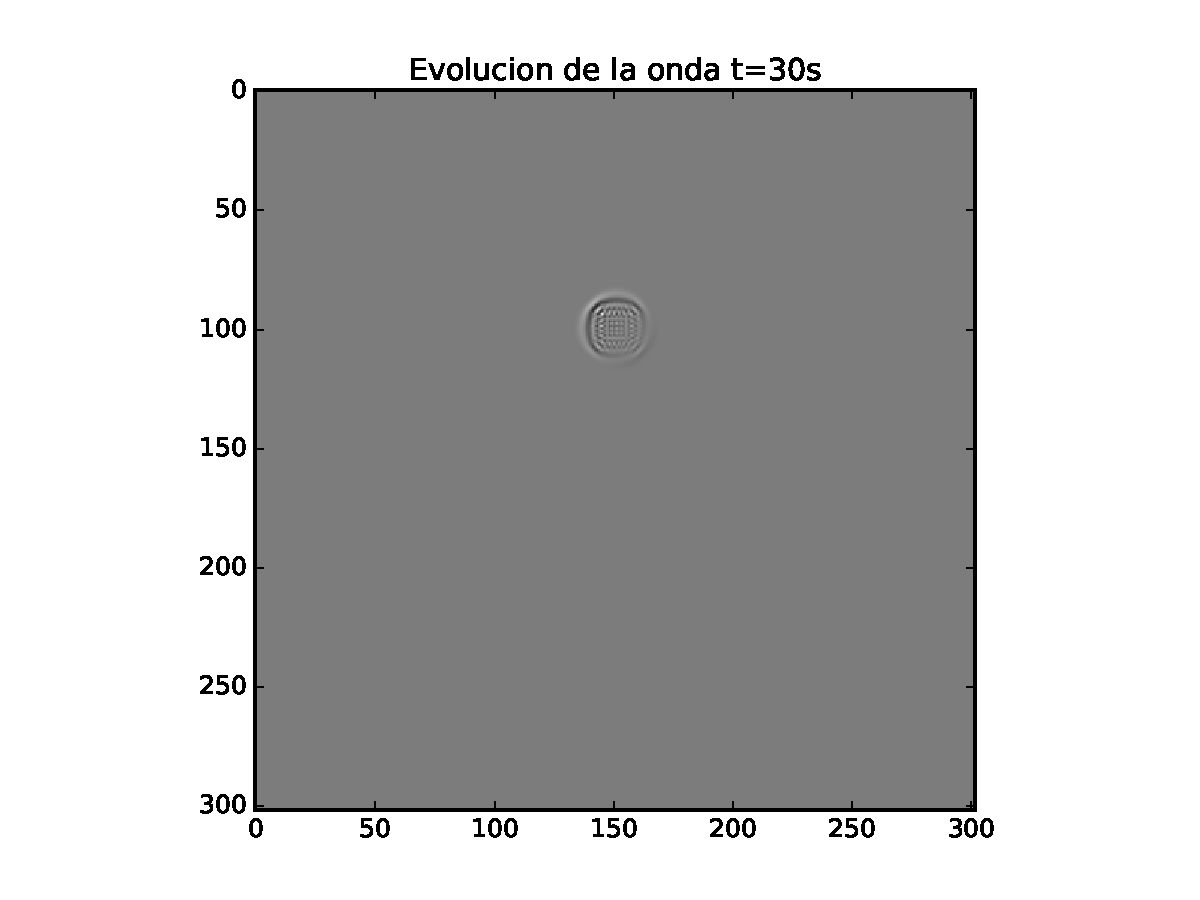
\includegraphics[width=0.7\textwidth]{Onda_30.png}
\caption{Propagacion de la onda en t=30s.}
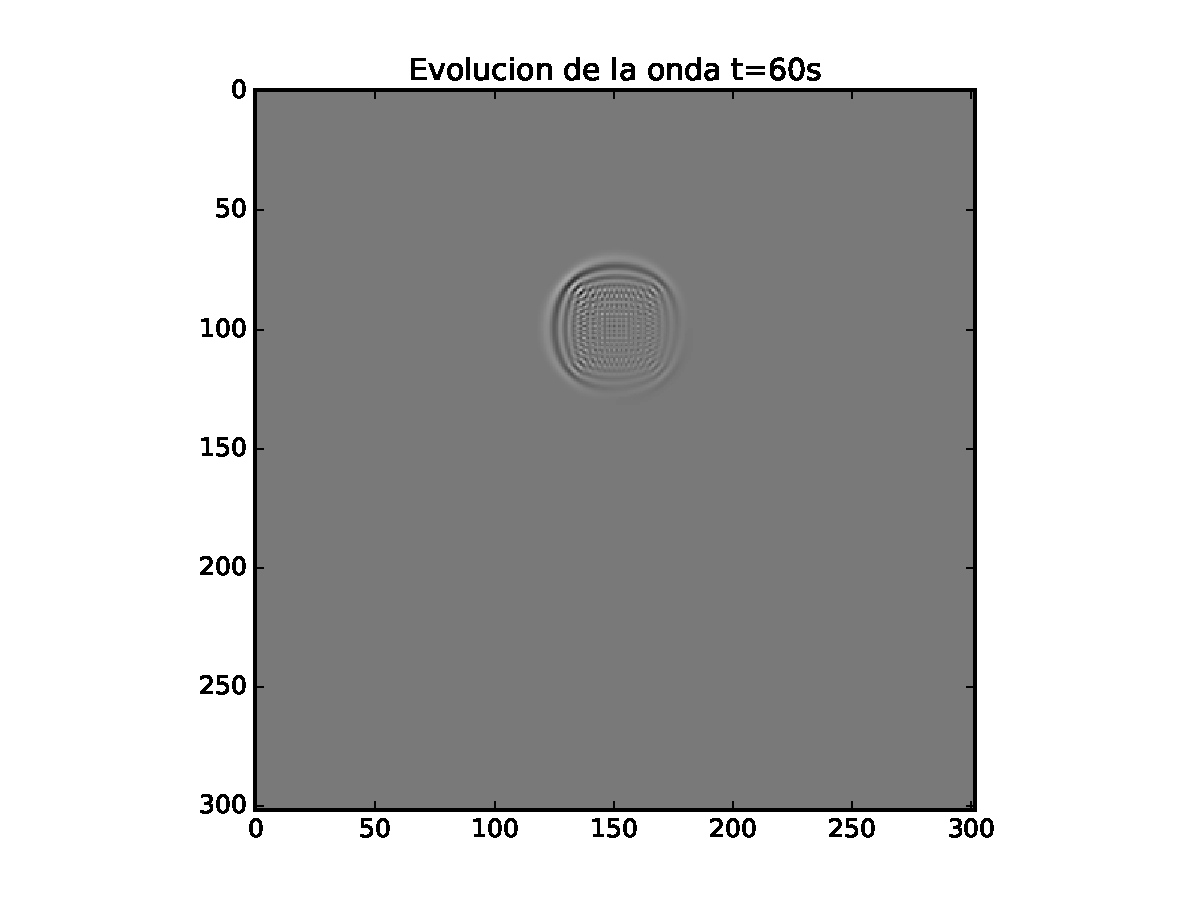
\includegraphics[width=0.7\textwidth]{Onda_60.png}
\caption{Propagacion de la onda en t=60s.}
\end{figure}

 
\section{Planetas}

En este ejercicio se busca conocer las orbitas de los planetas, en un tiempo de 250 años.
A partir de las condiciones iniciales dadas, se solucionó la ecuacion diferencial por el metodo de Leap Frog. 



\end{document}

